\chapter{Darah dan Sistem Peredaran}\label{ch:b2:blood-circulation}

Pada tahun 1628 William Harvey mengerjakan sebuah hitungan. Jantung,
menurut taksirannya, memuat kira-kira dua auns \omterm{def:b2:blood-circulation:blood}{darah} dan berdenyut tujuh
puluh kali tiap menit; sekalipun hanya sebagian kecil dari itu yang
diusir tiap denyutnya, jantungnya akan memompa dalam sejam beberapa
kali berat seluruh tubuhnya. \omterm{def:b2:blood-circulation:blood}{Darahnya} tidak mungkin dibuat lalu
dihabiskan dengan laju itu, seperti yang diajarkan Galenus selama empat
belas abad; ia pasti berputar dan berputar. Lalu ia menunjukkannya:
ikatkan seutas tali pada lengannya, maka \omterm{def:b2:blood-circulation:vessels}{vena} di bawah talinya
menggembung, bukan yang di atasnya; tekanlah \omterm{def:b2:blood-circulation:blood}{darah} di dalam sebuah \omterm{def:b2:blood-circulation:vessels}{vena}
menuju tangannya, melewati sebuah katup, dan ia tidak akan mau lewat.
\omterm{def:b2:blood-circulation:blood}{Darahnya} dipompa keluar lewat \omterm{def:b2:blood-circulation:vessels}{arteri}, kembali lewat \omterm{def:b2:blood-circulation:vessels}{vena}, dan seluruh
lima liternya melewati jantungnya tiap menit. Bab ini membahas sistem
tertutup itu --- apa \omterm{def:b2:blood-circulation:blood}{darahnya} itu, bagaimana ia dirutekan, fisika
alirannya lewat pembuluh dari aorta sampai sebuah \omterm{def:b2:blood-circulation:vessels}{kapiler}, dan
pertukaran, di dalam \omterm{def:b2:blood-circulation:vessels}{kapilernya}, yang menjadi tujuan semuanya itu.

\section{Darah}

\begin{definition}[Susunan darah]\label{def:b2:blood-circulation:blood}
\index{darah}\index{plasma}\index{hematokrit}\index{sel darah merah}\index{keping darah}
Darah adalah jaringan yang tersuspensi: kira-kira \qty{5}{L} pada
seorang dewasa, \qty{7}{\%} massa tubuhnya. Diputar sampai mengendap,
ia memisah menjadi \emph{plasma} (\qty{55}{\%}: air, \qty{70}{g/L}
protein --- albumin, globulin, fibrinogen --- beserta garam, gula,
lipid, gas, dan hormon yang ia bawa) dan sel (\qty{45}{\%}, yaitu
\emph{hematokrit}): \emph{sel darah merah} ($5\times 10^{12}$ tiap
liter, cakram bikonkaf \qty{7}{\micro m} tanpa nukleus, masing-masing
terjejali \num{280} juta molekul hemoglobin, hidup 120 hari dan dibuat
di dalam sumsum sebanyak dua juta tiap detik), \emph{sel darah putih}
($7\times 10^{9}$ tiap liter: neutrofil, limfosit, monosit, eosinofil,
basofil, yaitu lengan kekebalan yang bergerak), dan \emph{keping darah}
($3\times 10^{11}$ tiap liter, serpihan sel sumsum yang menyumbat luka
dan memulai pembekuan). Sel darah merahnya membawa oksigen ---
\qty{200}{mL} tiap liter darah pada kejenuhan penuh, tujuh puluh kali
yang dilarutkan air --- dan plasmanya membawa segala yang lain,
termasuk \qty{20}{\%} $\mathrm{CO_2}$ yang tidak berada di dalam
selnya, panas ototnya menuju kulitnya, dan hormon
\cref{ch:b2:cell-signalling} menuju sasarannya. Darah juga merupakan
larutan di bawah \emph{\omterm{thm:b2:blood-circulation:oncotic}{tekanan onkotik}}: proteinnya, yang tidak dapat
meninggalkan \omterm{def:b2:blood-circulation:vessels}{kapilernya}, menahan kira-kira \qty{25}{mmHg} tarikan
osmosis, dan tarikan itulah yang menjaga plasmanya tetap di dalam
pembuluhnya.
\end{definition}

\begin{omfigure}
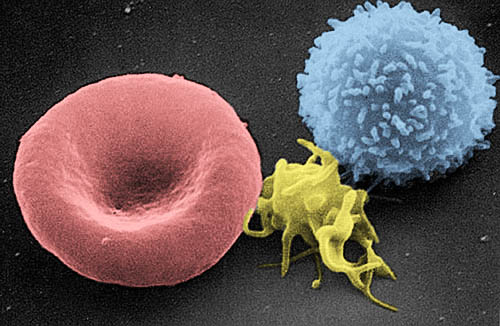
\includegraphics[width=0.5\linewidth]{images/book3/red-cells-nci.jpg}

{\small Sebuah \omterm{def:b2:blood-circulation:blood}{sel darah merah}, sebuah \omterm{def:b2:blood-circulation:blood}{keping darah}, dan sebuah sel
\omterm{def:b2:blood-circulation:blood}{darah} putih (sebuah limfosit) di bawah mikroskop elektron payar: ketiga
komponen berupa sel dari \omterm{def:b2:blood-circulation:blood}{darahnya}, digambar pada skala yang sama.}
\end{omfigure}

\begin{proposition}[Hemostasis]\label{prop:b2:blood-circulation:clotting}
\index{hemostasis}\index{riam pembekuan}\index{fibrin}
Sebuah pembuluh yang tersayat ditutup dalam tiga langkah dalam hitungan
menit. Pembuluhnya menyempit; \omterm{def:b2:blood-circulation:blood}{keping darahnya} melekat pada kolagen yang
tersingkap, melepaskan isyarat yang merekrut dan mengaktifkan lebih
banyak \omterm{def:b2:blood-circulation:blood}{keping darah}, lalu membentuk sebuah sumbat; dan sebuah
\emph{riam} protease \omterm{def:b2:blood-circulation:blood}{plasma}, yang masing-masing mengaktifkan yang
berikutnya (selusin faktor pembekuan, kebanyakan dibuat di dalam hati,
beberapa memerlukan vitamin K), mengubah fibrinogen menjadi
\emph{fibrin} yang tak larut, yang benangnya menganyam sumbatnya
menjadi sebuah beku \omterm{def:b2:blood-circulation:blood}{darah}. Sebuah riam memperkuat: setitik pemicunya
(faktor jaringan dari dinding yang rusak) berakhir pada berpuluh gram
fibrin. Ia juga harus dibendung: antikoagulan di dalam \omterm{def:b2:blood-circulation:blood}{plasmanya}
(antitrombin, protein C) dan pada endotelium yang utuh mengurung beku
\omterm{def:b2:blood-circulation:blood}{darahnya} pada lukanya, dan sebuah sistem kedua, fibrinolisis,
melarutkannya ketika pembuluhnya sembuh. Hemofilia adalah kekurangan
satu faktor; sebuah trombosis adalah beku \omterm{def:b2:blood-circulation:blood}{darah} di tempat yang tidak
menginginkannya, dan penyebab kematian terbesar di negeri yang kaya
adalah sebuah beku \omterm{def:b2:blood-circulation:blood}{darah} di dalam \omterm{def:b2:blood-circulation:vessels}{arteri} jantung atau otak.
\end{proposition}

\section{Rangkaian}

\begin{definition}[Terbuka dan tertutup, tunggal dan ganda]\label{def:b2:blood-circulation:circuits}
\index{peredaran terbuka}\index{peredaran tertutup}\index{peredaran ganda}%
\index{peredaran paru}\index{peredaran sistemik}
Pada sebuah peredaran \emph{terbuka} (serangga, kebanyakan moluska)
sebuah jantung memompa \omterm{def:b2:blood-circulation:blood}{darah} ke dalam sebuah rongga tubuh, tempat \omterm{def:b2:blood-circulation:blood}{darah}
itu memandikan organnya secara langsung lalu kembali pada tekanan yang
rendah; alirannya lambat dan buruk arahnya, dan serangga telah
memisahkan soal gasnya dari \omterm{def:b2:blood-circulation:blood}{darahnya} dengan memipakan udara langsung ke
jaringannya. Pada sebuah peredaran \emph{tertutup} (anelida, sefalopoda,
vertebrata) \omterm{def:b2:blood-circulation:blood}{darahnya} tetap berada di dalam pembuluh dan didorong lewat
\omterm{def:b2:blood-circulation:vessels}{kapiler} dengan tekanan, sehingga pembagiannya dapat dikendalikan organ
demi organ. Ikan memiliki satu rangkaian \emph{tunggal}: jantung $\to$
insang $\to$ tubuh $\to$ jantung, sehingga \omterm{def:b2:blood-circulation:blood}{darahnya} mencapai jaringannya
pada tekanan rendah yang tersisa setelah \omterm{def:b2:blood-circulation:vessels}{kapiler} insangnya. Mamalia dan
burung memiliki rangkaian \emph{ganda}: jantung kanannya menggerakkan
peredaran \emph{paru} (paru-paru, tekanan rendah, \qty{25}{mmHg}
sistolik) dan jantung kirinya, setelah \omterm{def:b2:blood-circulation:blood}{darahnya} kembali, menggerakkan
peredaran \emph{sistemik} (tubuh, tekanan tinggi, \qty{120}{mmHg});
kedua pompanya terpasang seri dan memindahkan aliran yang sama, yaitu
kira-kira \qty{5}{L} tiap menit ketika beristirahat. Amfibia dan
kebanyakan reptil memiliki jantung dengan satu bilik yang sebagian
mencampur kedua arusnya --- tahap antaranya. Rangkaian gandanya itulah
yang memungkinkan metabolisme berdarah panas: tekanan tinggi ke tiap
organ dan sebuah paru-paru yang terlindung darinya.
\end{definition}
\begin{proof}[Bukti eksperimental]
Harvey (1628) berhujah dari kuantitasnya --- keluaran yang dihitung di
atas --- dan dari strukturnya: katup di dalam \omterm{def:b2:blood-circulation:vessels}{vena}, yang telah
diperikan Fabricius, hanya membolehkan aliran menuju jantungnya,
sebagaimana ia tunjukkan dengan menekan \omterm{def:b2:blood-circulation:vessels}{vena} sebuah lengan yang
diikat; katup jantungnya hanya membolehkan aliran dari serambi ke bilik
lalu ke \omterm{def:b2:blood-circulation:vessels}{arteri}; dan \omterm{def:b2:blood-circulation:blood}{darah} di dalam \omterm{def:b2:blood-circulation:vessels}{arteri} menyembur, di dalam \omterm{def:b2:blood-circulation:vessels}{vena}
merembes. Ia tidak dapat melihat \omterm{def:b2:blood-circulation:vessels}{kapilernya} lalu menyimpulkannya;
Malpighi melihatnya di dalam paru-paru seekor katak pada tahun 1661,
empat tahun setelah Harvey wafat.
\end{proof}

\begin{omfigure}
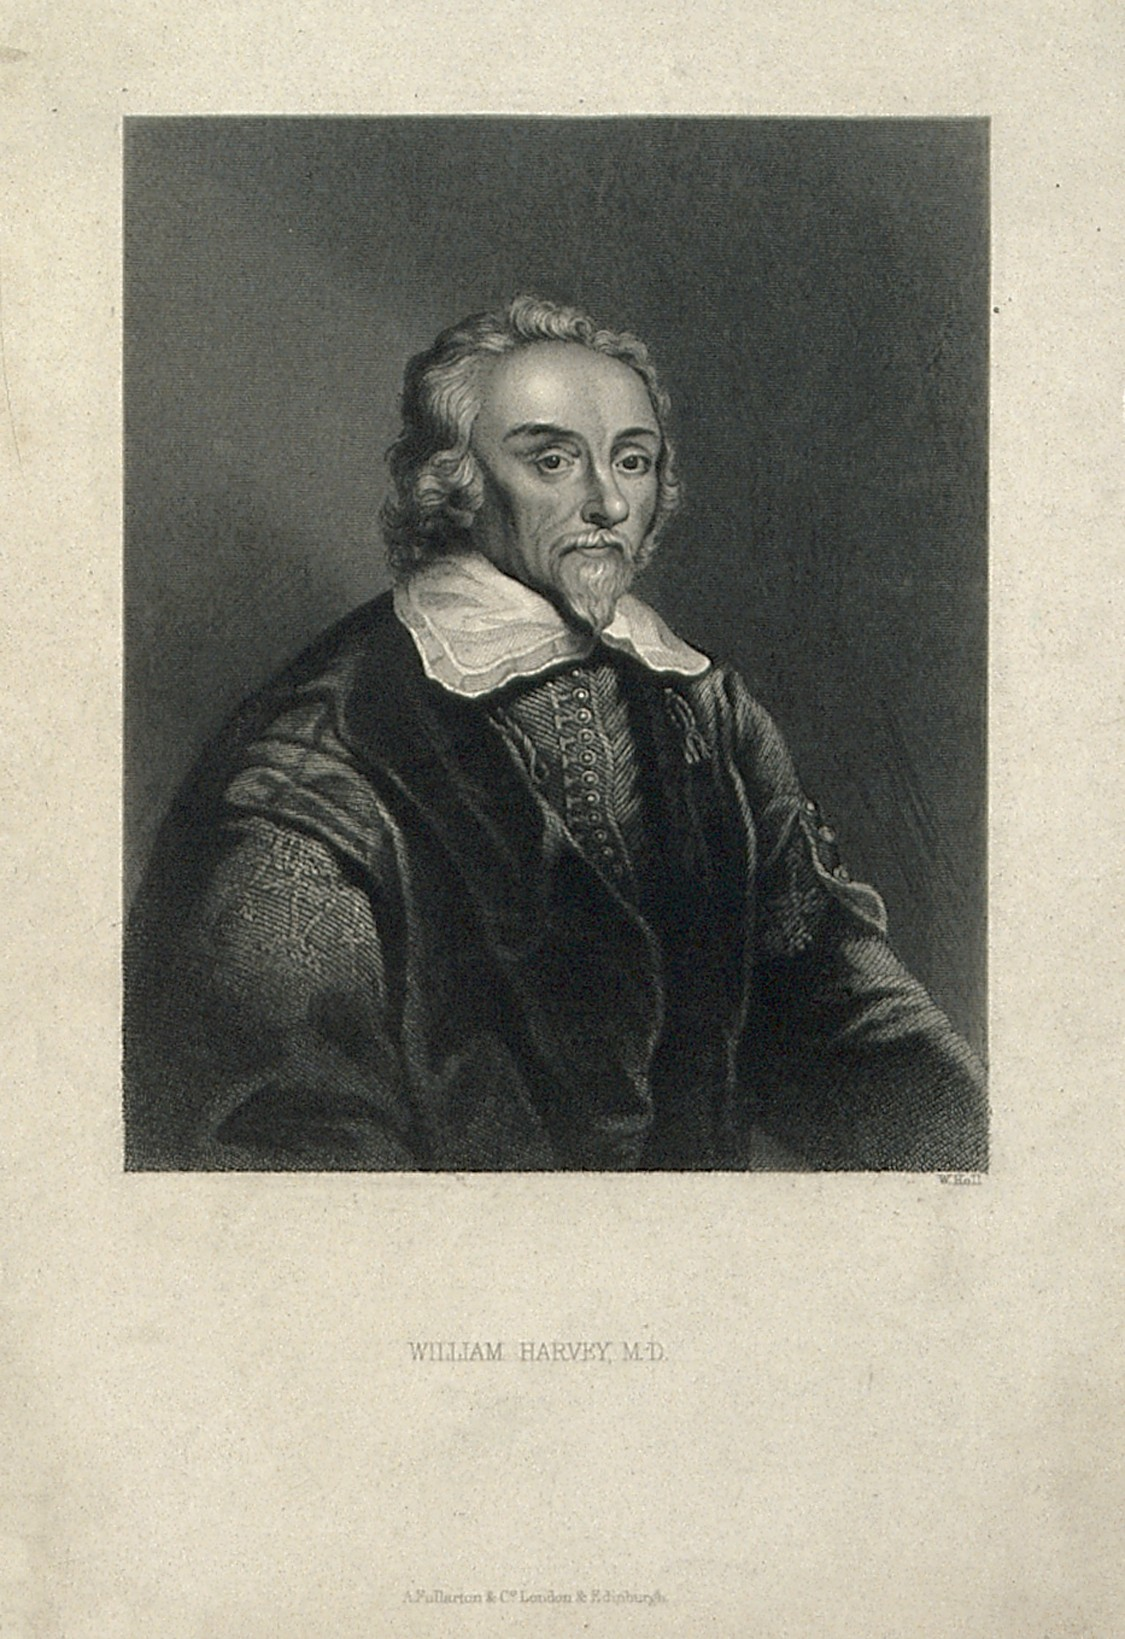
\includegraphics[width=0.3\linewidth]{images/book4/harvey.jpg}\hspace{0.05\linewidth}
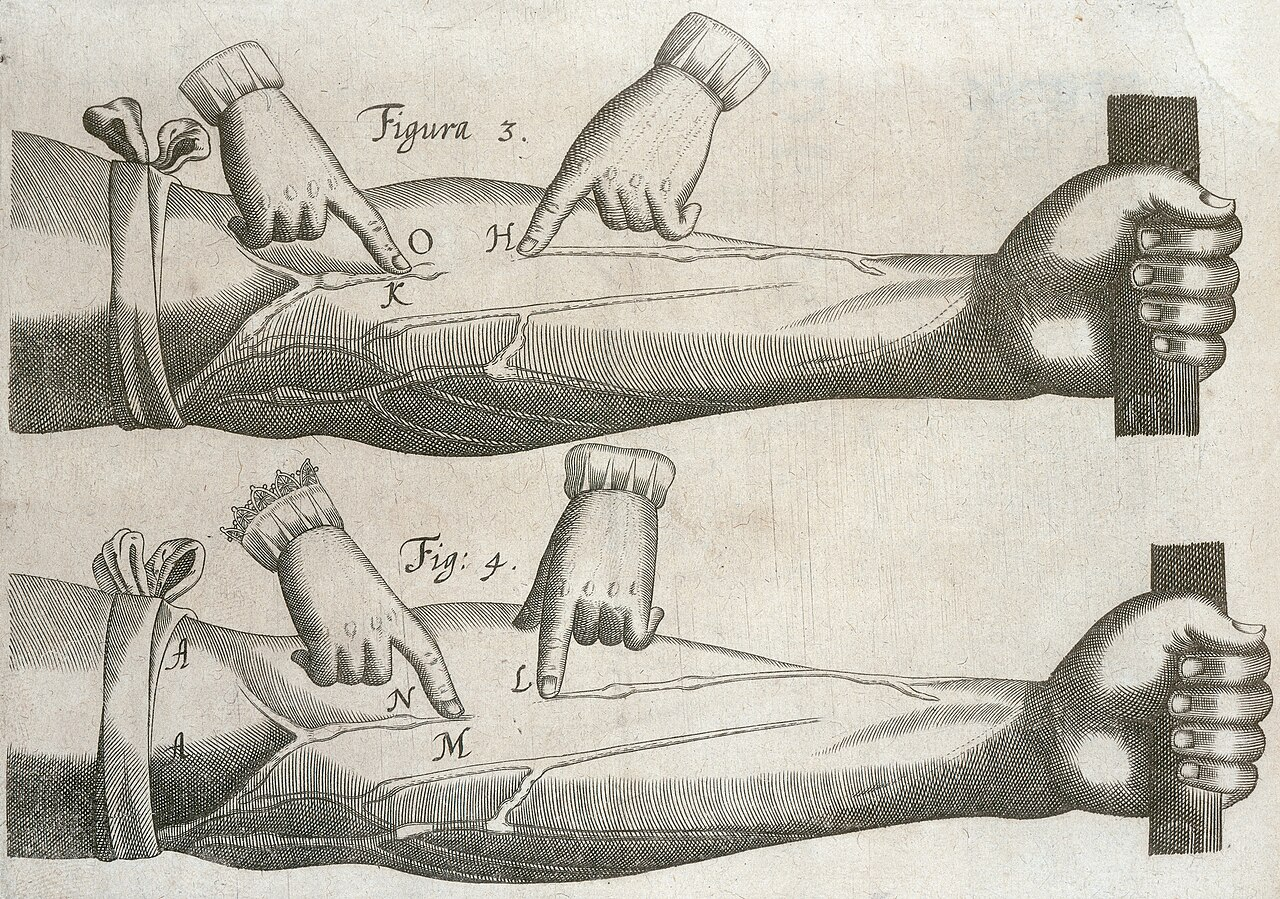
\includegraphics[width=0.42\linewidth]{images/book4/harvey-veins.jpg}

{\small William Harvey, dan plat dari bukunya tahun 1628: \omterm{def:b2:blood-circulation:vessels}{vena} sebuah
lengan bawah yang diikat menggembung di bawah talinya, dan \omterm{def:b2:blood-circulation:blood}{darah} yang
ditekan menuju tangannya berhenti pada katupnya.}
\end{omfigure}

\begin{omfigure}
\begin{tikzpicture}[every node/.style={font=\scriptsize}, >=stealth]
  % lungs and body
  \node[draw, rounded corners, fill=omDef!12, minimum width=3.4cm, minimum height=0.9cm] (lung) at (0,3) {paru-paru: kapiler paru};
  \node[draw, rounded corners, fill=omExo!25, minimum width=3.4cm, minimum height=0.9cm] (body) at (0,-3) {tubuh: kapiler sistemik};
  % heart chambers
  \node[draw, fill=omDef!25, minimum width=1.3cm, minimum height=0.7cm] (ra) at (-1.6,0.6) {serambi kanan};
  \node[draw, fill=omDef!35, minimum width=1.3cm, minimum height=0.9cm] (rv) at (-1.6,-0.5) {bilik kanan};
  \node[draw, fill=omThm!20, minimum width=1.3cm, minimum height=0.7cm] (la) at (1.6,0.6) {serambi kiri};
  \node[draw, fill=omThm!35, minimum width=1.3cm, minimum height=0.9cm] (lv) at (1.6,-0.5) {bilik kiri};
  \draw[->, thick] (ra) -- (rv); \draw[->, thick] (la) -- (lv);
  % pulmonary circuit
  \draw[->, very thick, omDef] (rv.west) -- ++(-1.4,0) |- (lung.west) node[pos=0.25, left, align=right] {arteri paru\\\qty{25}{mmHg}};
  \draw[->, very thick, omThm] (lung.east) -| (la.east) node[pos=0.75, right, align=left] {vena paru\\beroksigen};
  % systemic circuit
  \draw[->, very thick, omThm] (lv.east) -- ++(1.4,0) |- (body.east) node[pos=0.25, right, align=left] {aorta\\\qty{120}{mmHg}};
  \draw[->, very thick, omDef] (body.west) -| (ra.west);
  \node[omDef, anchor=east, align=right] at (-2.45,-1.6) {vena cava\\\qty{5}{mmHg}};
  \node[anchor=north, align=center] at (0,-3.7) {aliran yang sama lewat kedua rangkaiannya:\\\qty{5}{L/min} ketika beristirahat};
\end{tikzpicture}

{\small \omterm{def:b2:blood-circulation:circuits}{Peredaran gandanya}. Jantung kanan mengirim \omterm{def:b2:blood-circulation:blood}{darah} lewat
paru-parunya pada tekanan rendah; jantung kiri mengirimnya berkeliling
tubuhnya pada tekanan tinggi; kedua pompanya, yang terpasang seri,
memindahkan volume yang sama tiap menit.}
\end{omfigure}

\section{Pembuluh dan fisika alirannya}

\begin{definition}[Pohon pembuluhnya]\label{def:b2:blood-circulation:vessels}
\index{arteri}\index{arteriol}\index{kapiler}\index{vena}
\omterm{def:b2:blood-circulation:blood}{Darah} meninggalkan jantungnya lewat \emph{arteri}: tabung berdinding
tebal dengan lapisan elastik yang meregang tiap denyutnya dan mengerut
kembali di antara denyutnya, sehingga meratakan denyutnya menjadi
aliran yang lebih tunak (aorta bergaris tengah \qty{2.5}{cm}). Arteri
bercabang menjadi \emph{arteriol}, yaitu pembuluh sepersepuluh
milimeter atau kurang yang dindingnya sebagian besar berupa otot polos:
dengan berkerut atau mengendur, sebuah arteriol mengubah jari-jarinya
dan dengan demikian, secara dahsyat, hambatannya --- arteriol adalah
keran peredarannya dan tempat sebagian besar penurunan tekanannya.
Arteriol membuka ke dalam \emph{kapiler}: tabung yang terbuat dari satu
sel endotelium yang membungkus sebuah lumen \qtyrange{5}{10}{\micro m},
sepanjang kira-kira \qty{1}{mm}, sekitar empat puluh miliar banyaknya
dengan luas permukaan seluruhnya mendekati \qty{600}{m^2}, yang seluruh
pertukarannya berlangsung melintasi dindingnya. Kapiler mengalir ke
dalam venula dan \emph{vena}: berdinding tipis, dapat teregang, menahan
dua pertiga \omterm{def:b2:blood-circulation:blood}{darahnya} pada tekanan rendah, dengan katup yang menjaga
alirannya menuju jantungnya sementara otot memerasnya. Tiap pembuluh
dilapisi satu lapis \emph{endotelium}, yang bukan sebuah pelapis yang
pasif melainkan sebuah kelenjar --- ia melepaskan nitrogen monoksida
untuk mengendurkan arteriolnya, dan isyarat yang merekrut sel \omterm{def:b2:blood-circulation:blood}{darah}
putih --- sekaligus sebuah penapis.
\end{definition}

\begin{omfigure}
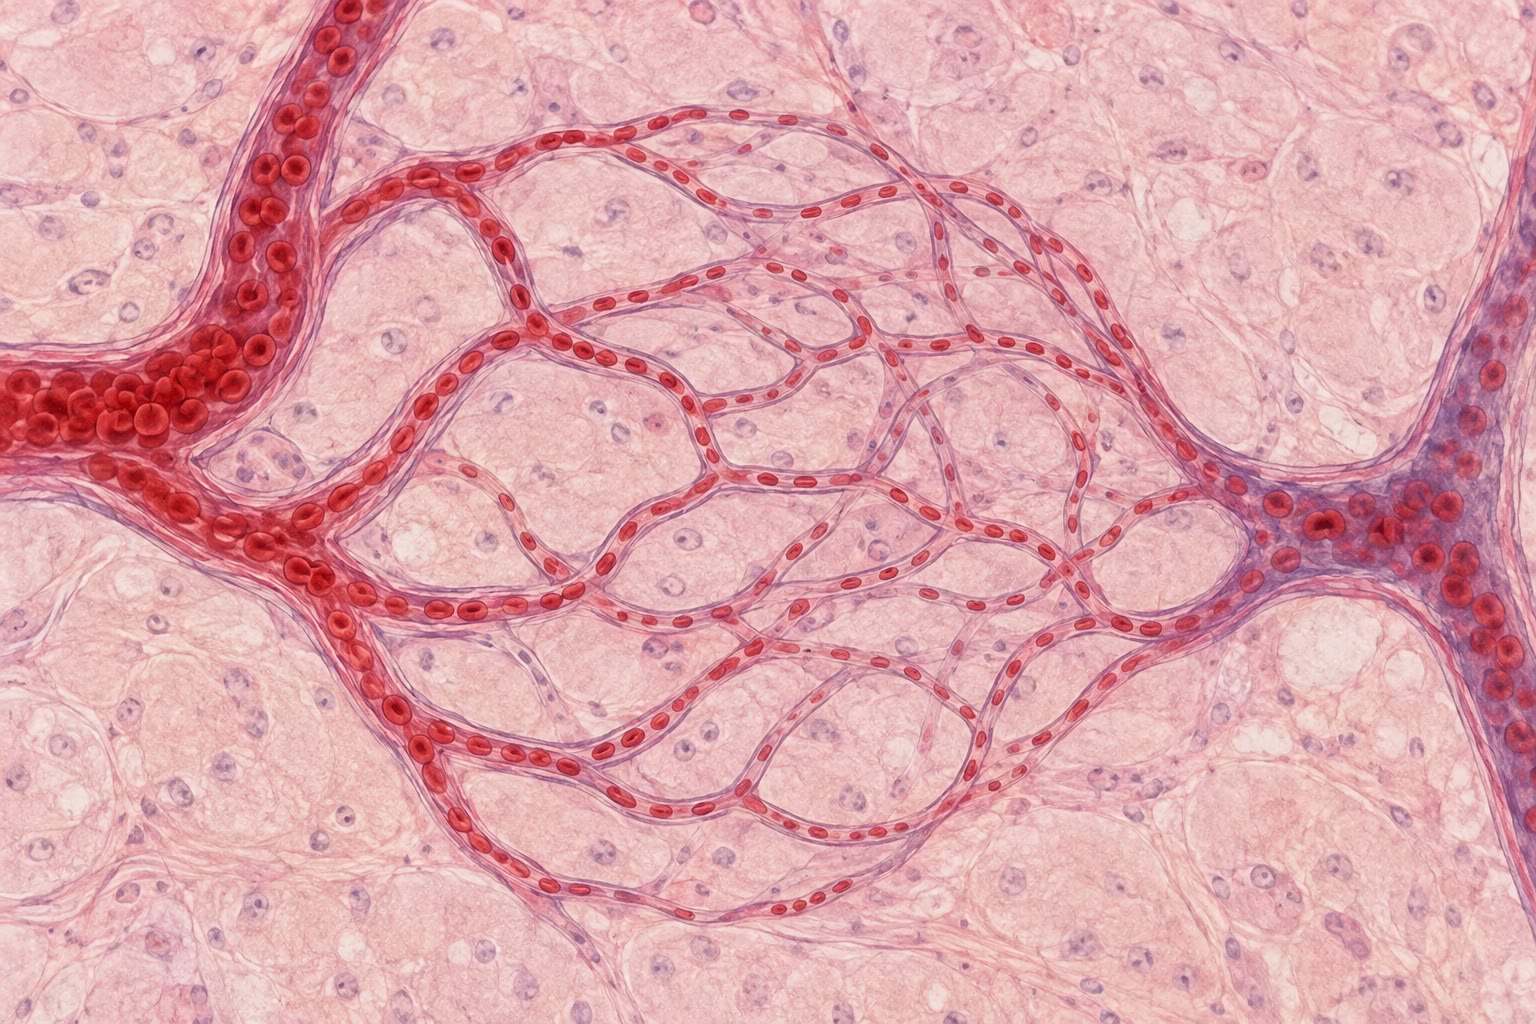
\includegraphics[width=0.55\linewidth]{images/book4/ai/b4-16-capillary-bed.jpg}

{\small Sebuah petak \omterm{def:b2:blood-circulation:vessels}{kapiler}: sebuah \omterm{def:b2:blood-circulation:vessels}{arteriol} yang memasok sebuah
anyaman \omterm{def:b2:blood-circulation:vessels}{kapiler}, yang di dalamnya \omterm{def:b2:blood-circulation:blood}{sel darah merah} berjalan satu per
satu, lalu bergabung kembali menjadi sebuah venula.}
\end{omfigure}

\begin{theorem}[Hukum Poiseuille dan hambatan pembuluh]\label{thm:b2:blood-circulation:poiseuille}
\index{hukum Poiseuille}\index{hambatan pembuluh}
Aliran tunak $Q$ sebuah fluida berkekentalan $\eta$ lewat sebuah tabung
berjari-jari $r$ dan berpanjang $L$ di bawah beda tekanan $\Delta P$
adalah
\[
Q = \frac{\pi r^{4}}{8\eta L}\,\Delta P, \qquad \text{sehingga}\qquad
R \equiv \frac{\Delta P}{Q} = \frac{8\eta L}{\pi r^{4}} .
\]
Hambatannya turun sebagai \emph{pangkat empat} jari-jarinya: sebuah
\omterm{def:b2:blood-circulation:vessels}{arteriol} yang menyempitkan jari-jarinya sebesar \qty{20}{\%}
melipatkan hambatannya dengan $1/0.8^{4} = 2.4$, dan yang
menyetengahkannya dengan 16. Itulah sebabnya beberapa milimeter otot
\omterm{def:b2:blood-circulation:vessels}{arteriol} dapat mengalihkan \omterm{def:b2:blood-circulation:blood}{darah} seluruh tubuhnya --- ke ususnya
setelah sebuah santapan, ke ototnya ketika berolahraga, ke kulitnya
ketika kepanasan --- dan sebabnya tekanannya turun dari \qty{95}{mmHg}
di dalam \omterm{def:b2:blood-circulation:vessels}{arteri} kecil menjadi \qty{35}{mmHg} pada pintu masuk
\omterm{def:b2:blood-circulation:vessels}{kapilernya}, hampir seluruhnya melintasi \omterm{def:b2:blood-circulation:vessels}{arteriolnya}, sedangkan
penurunan sepanjang aortanya hanya sepersekian milimeter raksa.
\end{theorem}
\begin{proof}
Pada aliran laminar yang tunak fluidanya bergerak dalam kulit yang
sepusat; gaya kental di antara kulitnya mengimbangi tekanannya. Bagi
silinder berjari-jari $s < r$ gaya tekan $\pi s^{2}\Delta P$ sama
dengan seretan kental pada permukaannya $2\pi s L\,\eta\,(-\mathrm{d}v/
\mathrm{d}s)$, sehingga $\mathrm{d}v/\mathrm{d}s = -s\Delta P/(2\eta L)$
dan, dengan $v(r) = 0$, $v(s) = (\Delta P/4\eta L)(r^{2} - s^{2})$ ---
sebuah tampang parabola. Dengan mengintegralkan kelajuannya pada
penampangnya,
$Q = \int_{0}^{r} v\,2\pi s\,\mathrm{d}s = (\pi\Delta P/2\eta L)
\int_{0}^{r}(r^{2}s - s^{3})\,\mathrm{d}s = \pi r^{4}\Delta P/8\eta
L$. (\omterm{def:b2:blood-circulation:blood}{Darah} tidak sepenuhnya merupakan fluida sederhana dan \omterm{def:b2:blood-circulation:vessels}{arteri}
tidaklah kaku, tetapi hukum pangkat empatnya berlaku cukup baik untuk
menjalankan sebuah tubuh.)
\end{proof}

\begin{theorem}[Keselanjaran: tempat darahnya melambat]\label{thm:b2:blood-circulation:continuity}
\index{persamaan keselanjaran}
Volume yang sama tiap detik melewati tiap aras pohonnya, sehingga
kelajuan rerata pada sebuah aras adalah $v = Q/A$, dengan $A$ adalah
luas penampang \emph{seluruh} pembuluh pada aras itu. Aorta
(\qty{3}{cm^2}) membawa \qty{5}{L/min} pada \qty{28}{cm/s}; \omterm{def:b2:blood-circulation:vessels}{kapilernya},
yang penampang seluruhnya mendekati \qty{3000}{cm^2}, membawanya pada
\qty{0.03}{cm/s}, sehingga sebuah \omterm{def:b2:blood-circulation:blood}{sel darah merah} memerlukan sekitar
tiga detik untuk melintasi sebuah \omterm{def:b2:blood-circulation:vessels}{kapiler} --- cukup waktu bagi
oksigennya untuk berdifusi keluar
(\cref{ch:b2:unicellular-diversity}: satu mikrometer dalam satu
milidetik). \omterm{def:b2:blood-circulation:vessels}{Vena}, yang penampang seluruhnya lebih kecil daripada
\omterm{def:b2:blood-circulation:vessels}{kapilernya}, mempercepat \omterm{def:b2:blood-circulation:blood}{darahnya} kembali menjadi \qty{10}{cm/s} di
dalam \omterm{def:b2:blood-circulation:vessels}{vena} cava. Pohonnya dibangun sedemikian rupa sehingga \omterm{def:b2:blood-circulation:blood}{darahnya}
lambat tepat di tempat ia harus bertukar dan cepat di tempat lainnya.
\end{theorem}
\begin{proof}
Kekekalan volume: apa yang masuk ke sebuah aras tiap detik
meninggalkannya, sehingga $Q = A\,v$ sama pada tiap aras. $\qty{5}{L/min} =
\qty{83}{cm^3/s}$; $83/3 = \qty{28}{cm/s}$; $83/3000 =
\qty{0.028}{cm/s}$.
\end{proof}

\begin{omfigure}
\begin{tikzpicture}
\begin{axis}[
  width=0.9\linewidth, height=6.4cm,
  axis x line=bottom, axis y line=left,
  xmin=0, xmax=7, ymin=0, ymax=130,
  xtick={0.5,1.5,2.5,3.5,4.5,5.5,6.5},
  xticklabels={aorta, arteri, arteriol, kapiler, venula, vena, vena cava},
  x tick label style={font=\scriptsize, rotate=30, anchor=north east},
  ylabel={tekanan (\unit{mmHg})}, ylabel style={font=\small, omThm},
  tick label style={font=\small}, ytick={0,40,80,120},
  legend style={font=\scriptsize, at={(0.97,0.95)}, anchor=north east, draw=none},
  clip=false,
]
\addplot[very thick, omThm] coordinates {(0,120) (0.5,118) (1,110) (1.5,100) (2,95) (2.5,60) (3,35) (3.5,25) (4,15) (4.5,12) (5,8) (5.5,5) (6,4) (6.5,3) (7,2)};
\addlegendentry{tekanan rerata}
\addplot[very thick, omThm, dashed] coordinates {(0,120) (0.5,120) (1,125) (1.5,120) (2,100)};
\addplot[very thick, omThm, dashed] coordinates {(0,80) (0.5,80) (1,80) (1.5,82) (2,88)};
\addlegendentry{sistolik dan diastolik}
\end{axis}
\begin{axis}[
  width=0.9\linewidth, height=6.4cm,
  axis x line=none, axis y line=right,
  xmin=0, xmax=7, ymin=0, ymax=32,
  ylabel={kelajuan (\unit{cm/s})}, ylabel style={font=\small, omDef},
  tick label style={font=\small}, ytick={0,10,20,30},
  legend style={font=\scriptsize, at={(0.97,0.72)}, anchor=north east, draw=none},
  clip=false,
]
\addplot[very thick, omDef] coordinates {(0,28) (0.5,26) (1,18) (1.5,10) (2,5) (2.5,1.5) (3,0.3) (3.5,0.03) (4,0.3) (4.5,1.5) (5,4) (5.5,7) (6,9) (6.5,10) (7,10)};
\addlegendentry{kelajuan rerata}
\end{axis}
\end{tikzpicture}

{\small Tekanan (merah) dan kelajuan rerata (biru) sepanjang \omterm{def:b2:blood-circulation:circuits}{peredaran
sistemiknya}. Denyutnya diratakan di dalam \omterm{def:b2:blood-circulation:vessels}{arterinya}, tekanannya turun
terutama melintasi \omterm{def:b2:blood-circulation:vessels}{arteriolnya}, dan \omterm{def:b2:blood-circulation:blood}{darahnya} paling lambat di dalam
\omterm{def:b2:blood-circulation:vessels}{kapilernya}, tempat penampang seluruhnya seribu kali penampang
aortanya.}
\end{omfigure}

\begin{theorem}[Arteri elastik sebagai tandon]\label{thm:b2:blood-circulation:windkessel}
\index{Windkessel}\index{komplians!arteri}\index{tekanan denyut}
Jantungnya menyemburkan dalam letupan; jaringannya menerima aliran yang
hampir tunak. \omterm{def:b2:blood-circulation:vessels}{Arteri} besarnya mengerjakan perataannya: \omterm{def:b2:blood-circulation:vessels}{arteri} itu
meregang selama semburannya, menyimpan sebagian volume sekuncupnya, lalu
mengerut kembali selama diastolnya, mendorongnya terus. Jika \omterm{def:b2:blood-circulation:vessels}{arterinya}
memiliki \emph{komplians} $C$ (volume yang tersimpan tiap satuan
tekanan) dan \omterm{def:b2:blood-circulation:vessels}{arteriolnya} sebuah hambatan $R$, maka selama diastolnya,
dengan katup aortanya tertutup, tekanannya meluruh sebagai
\[
P(t) = P_{s}\,e^{-t/RC},
\]
sehingga tekanan diastolik setelah sebuah diastol yang berlangsung
$t_d$ adalah $P_s e^{-t_d/RC}$: dengan $R = \qty{1}{mmHg.s/mL}$, $C =
\qty{2}{mL/mmHg}$, dan $t_d = \qty{0.8}{s}$, sebuah tekanan sistolik
\qty{120}{mmHg} turun menjadi \qty{80}{mmHg}. Aorta yang lebih kaku
($C$ yang lebih kecil, seperti pada usia tua) membiarkan tekanannya
turun lebih jauh di antara denyutnya dan naik lebih tinggi selama
semburannya: \emph{\omterm{thm:b2:blood-circulation:windkessel}{tekanan denyutnya}} melebar, dan jantungnya bekerja
melawan puncak yang lebih tinggi.
\end{theorem}
\begin{proof}
Selama diastolnya tidak ada \omterm{def:b2:blood-circulation:blood}{darah} yang masuk ke \omterm{def:b2:blood-circulation:vessels}{arterinya} dan \omterm{def:b2:blood-circulation:blood}{darah}
meninggalkannya lewat \omterm{def:b2:blood-circulation:vessels}{arteriolnya} pada $Q = P/R$; volume \omterm{def:b2:blood-circulation:vessels}{arterinya}
turun pada $\mathrm{d}V/\mathrm{d}t = -P/R$, dan karena $\mathrm{d}V = C\,
\mathrm{d}P$, $C\,\mathrm{d}P/\mathrm{d}t = -P/R$, yang penyelesaiannya
adalah eksponensial dengan tetapan waktu $RC$. Dengan $RC = \qty{2}{s}$:
$120\,e^{-0.4} = \qty{80}{mmHg}$.
\end{proof}

\section{Pertukaran di dalam kapilernya}

\begin{proposition}[Dua macam pertukaran]\label{prop:b2:blood-circulation:exchange}
\index{pertukaran kapiler}\index{gaya Starling}\index{edema}\index{getah bening}
Melintasi dinding \omterm{def:b2:blood-circulation:vessels}{kapilernya}, zat terlarut berpindah lewat
\emph{difusi} --- gas dan lipid lewat selnya, air dan zat terlarut
kecil lewat celah di antaranya, pada luas yang raksasa dan jarak yang
pendek yang membuat fluksnya berlimpah (hukum Fick, seperti pada
\omterm{def:b2:mammal-reproduction:placenta}{plasenta} pada \cref{ch:b2:mammal-reproduction}) --- dan air berpindah
lewat \emph{aliran ruah}, yang digerakkan oleh perimbangan dua tekanan.
Tekanan hidrostatik di dalam \omterm{def:b2:blood-circulation:vessels}{kapilernya}, $P_c$, mendorong cairannya
keluar; \omterm{thm:b2:blood-circulation:oncotic}{tekanan onkotik} protein \omterm{def:b2:blood-circulation:blood}{plasmanya}, $\pi_c$, menariknya masuk
(\emph{\omterm{prop:b2:blood-circulation:exchange}{gaya Starling}}). Pada ujung \omterm{def:b2:blood-circulation:vessels}{arterinya} $P_c \approx
\qty{35}{mmHg}$ melampaui $\pi_c \approx \qty{25}{mmHg}$ dan cairannya
tersaring keluar; pada ujung \omterm{def:b2:blood-circulation:vessels}{venanya} $P_c \approx \qty{15}{mmHg}$ dan
cairannya diserap kembali; pada seluruh tubuhnya kira-kira \qty{20}{L}
tiap hari tersaring keluar dan \qty{17}{L} kembali, dan sisa
\qty{3}{L}-nya, beserta protein yang bocor, dikumpulkan pembuluh
\emph{\omterm{prop:b2:blood-circulation:exchange}{getah bening}} lalu dikembalikan ke \omterm{def:b2:blood-circulation:vessels}{vena} di lehernya.
\emph{Edema} --- pembengkakan oleh cairan di dalam jaringannya ---
menyusul setiap kali perimbangannya berjungkit: tekanan \omterm{def:b2:blood-circulation:vessels}{vena} yang
tinggi (gagal jantung), protein \omterm{def:b2:blood-circulation:blood}{plasma} yang rendah (kelaparan, penyakit
hati atau ginjal), \omterm{def:b2:blood-circulation:vessels}{kapiler} yang bocor (radang), atau pembuluh \omterm{prop:b2:blood-circulation:exchange}{getah
bening} yang tersumbat.
\end{proposition}

\begin{omfigure}
\begin{tikzpicture}[every node/.style={font=\scriptsize}, >=stealth]
  % capillary
  \draw[thick, fill=omThm!10] (0,0) rectangle (9,1.2);
  \node[left] at (-0.1,0.6) {arteriol};
  \node[right] at (9.1,0.6) {venula};
  \draw[->, very thick, omThm] (0.3,0.6) -- (8.7,0.6);
  % pressures
  \node[above, align=center] at (1.5,1.3) {ujung arteri\\$P_c = 35$, $\pi_c = 25$};
  \node[above, align=center] at (7.5,1.3) {ujung vena\\$P_c = 15$, $\pi_c = 25$};
  \foreach \x in {0.8,1.5,2.2} \draw[->, thick, omDef] (\x,0) -- (\x,-0.7);
  \node[below, align=center, omDef] at (1.5,-0.75) {bersih $+10$ mmHg:\\penyaringan};
  \foreach \x in {6.8,7.5,8.2} \draw[->, thick, omDef] (\x,-0.7) -- (\x,0);
  \node[below, align=center, omDef] at (7.5,-0.75) {bersih $-10$ mmHg:\\penyerapan kembali};
  \draw[->, thick, omExo!70!black] (4.5,-0.4) -- (4.5,-1.6) node[below, align=center] {lebihnya ke getah bening:\\\qty{3}{L} tiap hari};
  \node[align=center] at (4.5,-0.15) {cairan antarsel};
\end{tikzpicture}

{\small \omterm{prop:b2:blood-circulation:exchange}{Gaya Starling} sepanjang sebuah \omterm{def:b2:blood-circulation:vessels}{kapiler}. Tekanan hidrostatik
mendorong cairannya keluar dan \omterm{thm:b2:blood-circulation:oncotic}{tekanan onkotik} protein \omterm{def:b2:blood-circulation:blood}{plasmanya}
menariknya kembali; penyaringan pada ujung \omterm{def:b2:blood-circulation:vessels}{arterinya} melampaui
penyerapan kembali pada ujung \omterm{def:b2:blood-circulation:vessels}{venanya}, dan \omterm{prop:b2:blood-circulation:exchange}{getah beningnya}
mengembalikan selisihnya.}
\end{omfigure}

\begin{theorem}[Tekanan onkotik]\label{thm:b2:blood-circulation:oncotic}
\index{tekanan onkotik}\index{albumin}
Sebuah larutan berisi $c$ mol tiap liter zat terlarut yang tidak dapat
menyeberangi sebuah membran mengerahkan melintasinya sebuah tekanan
osmosis $\pi = cRT$ (van 't Hoff). Albumin \omterm{def:b2:blood-circulation:blood}{plasma}, yaitu \qty{40}{g/L}
sebuah protein bermassa molar \qty{66}{kg/mol}, adalah $c = \qty{0.6}{mmol/L}$ dan memberikan $\pi =
0.6\times 8.314\times 310 = \qty{1.55}{kPa} \approx \qty{12}{mmHg}$; protein lainnya beserta ion
tambahan yang ditahan muatan negatif albuminnya membawa jumlahnya
menjadi kira-kira \qty{25}{mmHg}. Natrium klorida \omterm{def:b2:blood-circulation:blood}{plasmanya}, pada
\qty{150}{mmol/L}, akan mengerahkan \qty{5800}{mmHg} --- tetapi ia
menyeberangi dinding \omterm{def:b2:blood-circulation:vessels}{kapilernya} dengan bebas dan tidak mengerahkan apa
pun melintasinya. Yang penting bagi \omterm{def:b2:blood-circulation:vessels}{kapilernya} adalah proteinnya:
setengahkan albuminnya, seperti pada penyakit ginjal yang
kehilangannya lewat air seni, maka tarikan penyerapnya menyetengah,
cairannya menumpuk di dalam jaringannya, dan pasiennya membengkak.
\end{theorem}
\begin{proof}
$\qty{40}{g/L}/\qty{66000}{g/mol} = \qty{6.1e-4}{mol/L} =
\qty{0.61}{mol/m^3}$; $\pi = cRT = 0.61\times 8.314\times 310 =
\qty{1570}{Pa}$; $\qty{1}{mmHg} = \qty{133}{Pa}$, sehingga \qty{11.8}{mmHg}.
Hukum van 't Hoff itu sendiri adalah limit larutan encer yang
diturunkan di dalam jilid Tahun 1.
\end{proof}

\begin{example}[Peredarannya sebagai sistem angkutan]\label{ex:b2:blood-circulation:transport}
Lima liter tiap menit lewat \qty{600}{m^2} dinding \omterm{def:b2:blood-circulation:vessels}{kapiler} adalah
sebuah jasa antaran yang tiada bandingnya. Ia membawakan tiap selnya
oksigen dalam jarak beberapa garis tengah sel (tidak ada sel tubuhnya
yang berjarak lebih dari \qty{20}{\micro m} dari sebuah \omterm{def:b2:blood-circulation:vessels}{kapiler}),
menyingkirkan $\mathrm{CO_2}$, laktat, dan ureanya, membawa glukosa
hatinya ke otaknya dan asam lemak simpanan lemaknya ke ototnya,
menyebarkan hormon \cref{ch:b2:cell-signalling} dari satu kelenjar ke
tiap reseptor di dalam tubuhnya dalam semenit, memindahkan panas
intinya ke kulitnya lalu kembali, dan mengantarkan sel \omterm{def:b2:blood-circulation:blood}{darah} putihnya
ke sebuah luka dalam hitungan jam. Ia juga merupakan kerawanannya:
sebuah beku \omterm{def:b2:blood-circulation:blood}{darah}, sebuah pendarahan, atau sebuah pompa yang gagal
menghentikan semuanya sekaligus, dan otaknya, yang tidak menyimpan
bahan bakar, gagal dalam hitungan detik. Sisa bagian buku ini membahas
pompanya (\cref{ch:b2:heart}) dan bagaimana tekanannya diatur sehingga
jasanya berlanjut sepanjang berdiri, berlari, dan berdarah
(\cref{ch:b2:blood-pressure}).
\end{example}

\section{Latihan}

\begin{exercise}[$\star$]\label{exo:b2:blood-circulation:1}
Berikan susunan \omterm{def:b2:blood-circulation:blood}{darah} menurut volumenya beserta jumlah, ukuran, dan
fungsi tiap komponennya yang berupa sel.
\end{exercise}

\begin{exercise}[$\star$]\label{exo:b2:blood-circulation:2}
Gambarlah rangkaian seekor ikan dan seekor mamalia, tandai tekanannya,
dan katakan apa yang diperoleh rangkaian gandanya.
\end{exercise}

\begin{exercise}[$\star$]\label{exo:b2:blood-circulation:3}
Bagi tiap jenis pembuluh --- \omterm{def:b2:blood-circulation:vessels}{arteri}, \omterm{def:b2:blood-circulation:vessels}{arteriol}, \omterm{def:b2:blood-circulation:vessels}{kapiler}, \omterm{def:b2:blood-circulation:vessels}{vena} ---
berikan struktur dindingnya dan fungsi yang ia layani.
\end{exercise}

\begin{exercise}[$\star$]\label{exo:b2:blood-circulation:4}
Bangunlah kembali hujah Harvey dari kuantitasnya, dengan angka modern:
\qty{70}{mL} tiap denyut, \num{72} denyut tiap menit, \qty{5}{L} \omterm{def:b2:blood-circulation:blood}{darah}.
\end{exercise}

\begin{exercise}[$\star\star$]\label{exo:b2:blood-circulation:5}
Hitunglah penurunan tekanan sepanjang aortanya (jari-jari
\qty{1.25}{cm}, panjang \qty{40}{cm}, $\eta = \qty{3e-3}{Pa.s}$) yang
membawa \qty{5}{L/min} dengan \omterm{thm:b2:blood-circulation:poiseuille}{hukum Poiseuille}, dalam pascal dan dalam mmHg. Berilah ulasan.
\end{exercise}

\begin{exercise}[$\star\star$]\label{exo:b2:blood-circulation:6}
Sebuah \omterm{def:b2:blood-circulation:vessels}{arteriol} berjari-jari \qty{15}{\micro m} menyempit menjadi
\qty{12}{\micro m}, lalu melebar menjadi \qty{20}{\micro m}. Dengan
faktor berapa hambatannya berubah pada tiap keadaannya, dan alirannya
pada tekanan yang tetap?
\end{exercise}

\begin{exercise}[$\star\star$]\label{exo:b2:blood-circulation:7}
Aorta memiliki penampang \qty{3}{cm^2} dan \omterm{def:b2:blood-circulation:vessels}{kapilernya} seluruhnya
\qty{3000}{cm^2}; alirannya \qty{5}{L/min}. Hitunglah kelajuan rerata
pada masing-masingnya, dan waktu yang dihabiskan sebuah \omterm{def:b2:blood-circulation:blood}{sel darah merah}
di dalam sebuah \omterm{def:b2:blood-circulation:vessels}{kapiler} \qty{1}{mm}. Ketika berolahraga keluarannya
naik menjadi \qty{25}{L/min} dan \omterm{def:b2:blood-circulation:vessels}{kapiler} ototnya membuka: apa yang
terjadi pada waktu lintasnya?
\end{exercise}

\begin{exercise}[$\star\star$]\label{exo:b2:blood-circulation:8}
Dengan $P_c = 35$ dan \qty{15}{mmHg} pada kedua ujungnya, $\pi_c =
\qty{25}{mmHg}$, dan tekanan antarselnya diabaikan, hitunglah tekanan
penyaringan bersih pada tiap ujungnya. Apa yang terjadi jika tekanan
\omterm{def:b2:blood-circulation:vessels}{venanya} naik sehingga $P_c$ pada ujung \omterm{def:b2:blood-circulation:vessels}{venanya} menjadi \qty{28}{mmHg}?
\end{exercise}

\begin{exercise}[$\star\star$]\label{exo:b2:blood-circulation:9}
Hitunglah \omterm{thm:b2:blood-circulation:oncotic}{tekanan onkotik} \qty{40}{g/L} albumin (\qty{66}{kg/mol}) pada
\qty{37}{\celsius}, dan \qty{20}{g/L}. Mengapa natrium \omterm{def:b2:blood-circulation:blood}{plasmanya}, pada
\qty{150}{mmol/L}, tidak menyumbang apa pun kepada perimbangan
Starlingnya?
\end{exercise}

\begin{exercise}[$\star\star\star$]\label{exo:b2:blood-circulation:10}
Dengan $R = \qty{1}{mmHg.s/mL}$ dan $C = \qty{2}{mL/mmHg}$, hitunglah
tekanan diastolik setelah \qty{0.8}{s} dari sebuah tekanan sistolik
\qty{120}{mmHg}. Hitung ulang bagi aorta yang kompliansnya setengahnya.
Jelaskan mengapa \omterm{thm:b2:blood-circulation:windkessel}{tekanan denyut} orang lanjut usia melebar, dan apa
ongkosnya bagi jantungnya.
\end{exercise}

\begin{exercise}[$\star\star\star$]\label{exo:b2:blood-circulation:11}
Hambatan sistemiknya adalah $R = (P_{\text{art}} - P_{\text{ven}})/Q$.
Hitunglah ia ketika beristirahat ($95 - 5$ mmHg, \qty{5}{L/min}) dan
ketika berolahraga ($110 - 5$, \qty{25}{L/min}). Dengan faktor berapa
jari-jari \omterm{def:b2:blood-circulation:vessels}{arteriol} reratanya pasti telah berubah, jika \omterm{def:b2:blood-circulation:vessels}{arteriolnya}
memikul seluruh hambatannya?
\end{exercise}

\begin{exercise}[$\star\star\star$]\label{exo:b2:blood-circulation:12}
``Peredarannya dibangun sedemikian rupa sehingga \omterm{def:b2:blood-circulation:blood}{darahnya} lambat di
tempat ia harus bertukar dan cepat di tempat lainnya.'' Bahaslah,
dengan \omterm{thm:b2:blood-circulation:continuity}{persamaan keselanjaran}, \omterm{thm:b2:blood-circulation:poiseuille}{hukum Poiseuille}, dan geometri pohonnya,
dan katakan mengapa sebuah \omterm{def:b2:blood-circulation:circuits}{peredaran terbuka} tidak dapat berbuat sama.
\end{exercise}

\section{Soal: Peredarannya dalam Angka}

\begin{problem}[{Soal akhir pekan --- hitungan Harvey dikerjakan ulang,
tekanan dan kelajuan pohon pembuluhnya dihitung dengan Poiseuille dan
keselanjaran, penyaringan harian kapilernya diimbangkan, dan perataan
oleh aortanya dimodelkan, berakhir pada curah jantungnya, penurunan
tekanan arteriolnya, saringan hariannya, dan tekanan diastoliknya}]
\label{pb:b2:blood-circulation:1}
Datanya: volume sekuncup \qty{70}{mL}, laju denyut \qty{72}{min^{-1}},
volume \omterm{def:b2:blood-circulation:blood}{darah} \qty{5}{L}, $\eta = \qty{3e-3}{Pa.s}$, $\qty{1}{mmHg} =
\qty{133}{Pa}$. Aorta: jari-jari \qty{1.25}{cm}, panjang \qty{40}{cm}.
\omterm{def:b2:blood-circulation:vessels}{Arteriol}: $3\times 10^{6}$ terpasang sejajar, masing-masing berjari-jari
\qty{15}{\micro m} dan berpanjang \qty{1}{mm}. \omterm{def:b2:blood-circulation:vessels}{Kapiler}: $4\times
10^{10}$, jari-jari \qty{3}{\micro m}, panjang \qty{1}{mm}, seperempatnya
terbuka ketika beristirahat. Starling: $P_c$ dari 35 menjadi \qty{15}{mmHg}
sepanjang sebuah \omterm{def:b2:blood-circulation:vessels}{kapiler}, $\pi_c = \qty{25}{mmHg}$. Windkessel: $C =
\qty{2}{mL/mmHg}$, diastol \qty{0.8}{s}.

\medskip
\noindent\textbf{Bagian I --- Hitungan Harvey.}
\begin{enumerate}
  \item Hitunglah curah jantungnya dalam liter tiap menit dan tiap hari.
  \item Berapa kali volume \omterm{def:b2:blood-circulation:blood}{darahnya} beredar dalam sehari?
  \item Taksiran Harvey adalah 2~auns (\qty{57}{g}) tiap denyut, yang
        menurut dugaannya sekurang-kurangnya seperempatnya diusir, pada
        72 denyut tiap menit. Massa \omterm{def:b2:blood-circulation:blood}{darah} berapa yang diberikannya tiap
        jam, dan bagaimana perbandingannya dengan berat seorang lelaki?
  \item Mengapa ini merupakan hujah bagi peredarannya alih-alih bagi
        pembuatan dan pemakaian yang menerus?
  \item Perikan percobaan pengikatannya dan apa yang ditunjukkan katupnya.
  \item Apa yang tidak dapat dilihat Harvey, dan siapa yang melihatnya?
\end{enumerate}

\medskip
\noindent\textbf{Bagian II --- Pohonnya.}
\begin{enumerate}[resume]
  \item Hitunglah kelajuan rerata di dalam aortanya.
  \item Hitunglah penurunan tekanan sepanjang aortanya dengan \omterm{thm:b2:blood-circulation:poiseuille}{hukum
        Poiseuille}, dalam mmHg.
  \item Hitunglah hambatan satu \omterm{def:b2:blood-circulation:vessels}{arteriol} dan hambatan $3\times
        10^{6}$ yang terpasang sejajar.
  \item Hitunglah penurunan tekanan melintasi \omterm{def:b2:blood-circulation:vessels}{arteriolnya} pada
        keluaran ketika beristirahat, dalam mmHg.
  \item Hitunglah penampang seluruh \omterm{def:b2:blood-circulation:vessels}{kapiler} yang terbuka dan kelajuan
        rerata di dalamnya; lalu waktu lintas lewat salah satunya.
  \item \omterm{def:b2:blood-circulation:vessels}{Arteriolnya} menyempit sehingga jari-jarinya turun sebesar
        \qty{10}{\%}. Hitung ulang penurunannya. Apa yang harus
        dikerjakan jantungnya untuk menjaga keluaran yang sama?
\end{enumerate}

\medskip
\noindent\textbf{Bagian III --- \omterm{def:b2:blood-circulation:vessels}{Kapilernya}.}
\begin{enumerate}[resume]
  \item Hitunglah tekanan penyaringan bersih pada ujung \omterm{def:b2:blood-circulation:vessels}{arterinya},
        pada ujung \omterm{def:b2:blood-circulation:vessels}{venanya}, dan pada titik tengahnya (anggaplah $P_c$
        turun secara lurus).
  \item Belahlah \omterm{def:b2:blood-circulation:vessels}{kapilernya} menjadi separuh yang menyaring dan separuh
        yang menyerap kembali lalu taksirlah cairan yang tersaring dan
        terserap kembali tiap hari pada seluruh tubuhnya, dengan
        mengambil tekanan bersih yang direratakan pada tiap separuhnya
        sebagai $+10$ dan \qty{-8.5}{mmHg} dan tiap separuhnya
        memindahkan \qty{2}{L} tiap hari tiap mmHg.
  \item Simpulkan aliran \omterm{prop:b2:blood-circulation:exchange}{getah beningnya}.
  \item Albumin \omterm{def:b2:blood-circulation:blood}{plasmanya} turun menjadi \qty{20}{g/L}. Hitung ulang
        $\pi_c$ (anggaplah ia berskala dengan albuminnya) dan tekanan
        bersih pada kedua ujungnya. Apa yang terjadi?
  \item Tekanan \omterm{def:b2:blood-circulation:vessels}{venanya} naik sehingga $P_c$ berjalan dari 35 menjadi
        \qty{28}{mmHg}. Hitung ulang tekanan bersih reratanya dan
        perimbangan hariannya. Ke mana cairannya pergi?
  \item Hitunglah permukaan seluruh \omterm{def:b2:blood-circulation:vessels}{kapilernya} (silinder, semuanya) dan
        waktu yang diperlukan sebuah molekul untuk berdifusi ke sebuah
        sel yang berjarak \qty{20}{\micro m} dari sebuah \omterm{def:b2:blood-circulation:vessels}{kapiler} ($D = \qty{1e-9}{m^2/s}$).
\end{enumerate}

\medskip
\noindent\textbf{Bagian IV --- Aortanya sebagai tandon.}
\begin{enumerate}[resume]
  \item Hitunglah hambatan sistemiknya dari tekanan rerata
        \qty{93}{mmHg}, tekanan \omterm{def:b2:blood-circulation:vessels}{vena} \qty{3}{mmHg}, dan keluaran ketika
        beristirahat, dalam \unit{mmHg.s/mL}.
  \item Hitunglah tetapan waktu $RC$ dan tekanan diastolik setelah
        \qty{0.8}{s} dari sebuah tekanan sistolik \qty{120}{mmHg}.
  \item Hitung ulang bagi $C = \qty{1}{mL/mmHg}$. Apa yang terjadi pada
        \omterm{thm:b2:blood-circulation:windkessel}{tekanan denyutnya}?
  \item Laju denyutnya naik menjadi \num{120} dan diastolnya memendek
        menjadi \qty{0.3}{s}. Hitunglah tekanan diastoliknya.
  \item Dari \qty{70}{mL} yang disemburkan, berapa banyak yang tersimpan
        di dalam \omterm{def:b2:blood-circulation:vessels}{arterinya} selama sistolnya jika tekanannya naik sebesar
        \qty{20}{mmHg}? Ke mana sisanya pergi?
  \item Jelaskan mengapa \omterm{def:b2:blood-circulation:vessels}{arteri} jantungnya, yang terisi pada diastolnya,
        bergantung pada kerutan balik aortanya.
  \item Nyatakan hasilnya: curah jantungnya, penurunan tekanan
        \omterm{def:b2:blood-circulation:vessels}{arteriolnya}, saringan bersih hariannya, dan tekanan diastoliknya
        bagi $C = 2$ dan $C = 1$.
\end{enumerate}
\end{problem}
